\section{Reference-Guided Merge Tree Maps}\label{sec:method}
\begin{figure*}[t]
\centering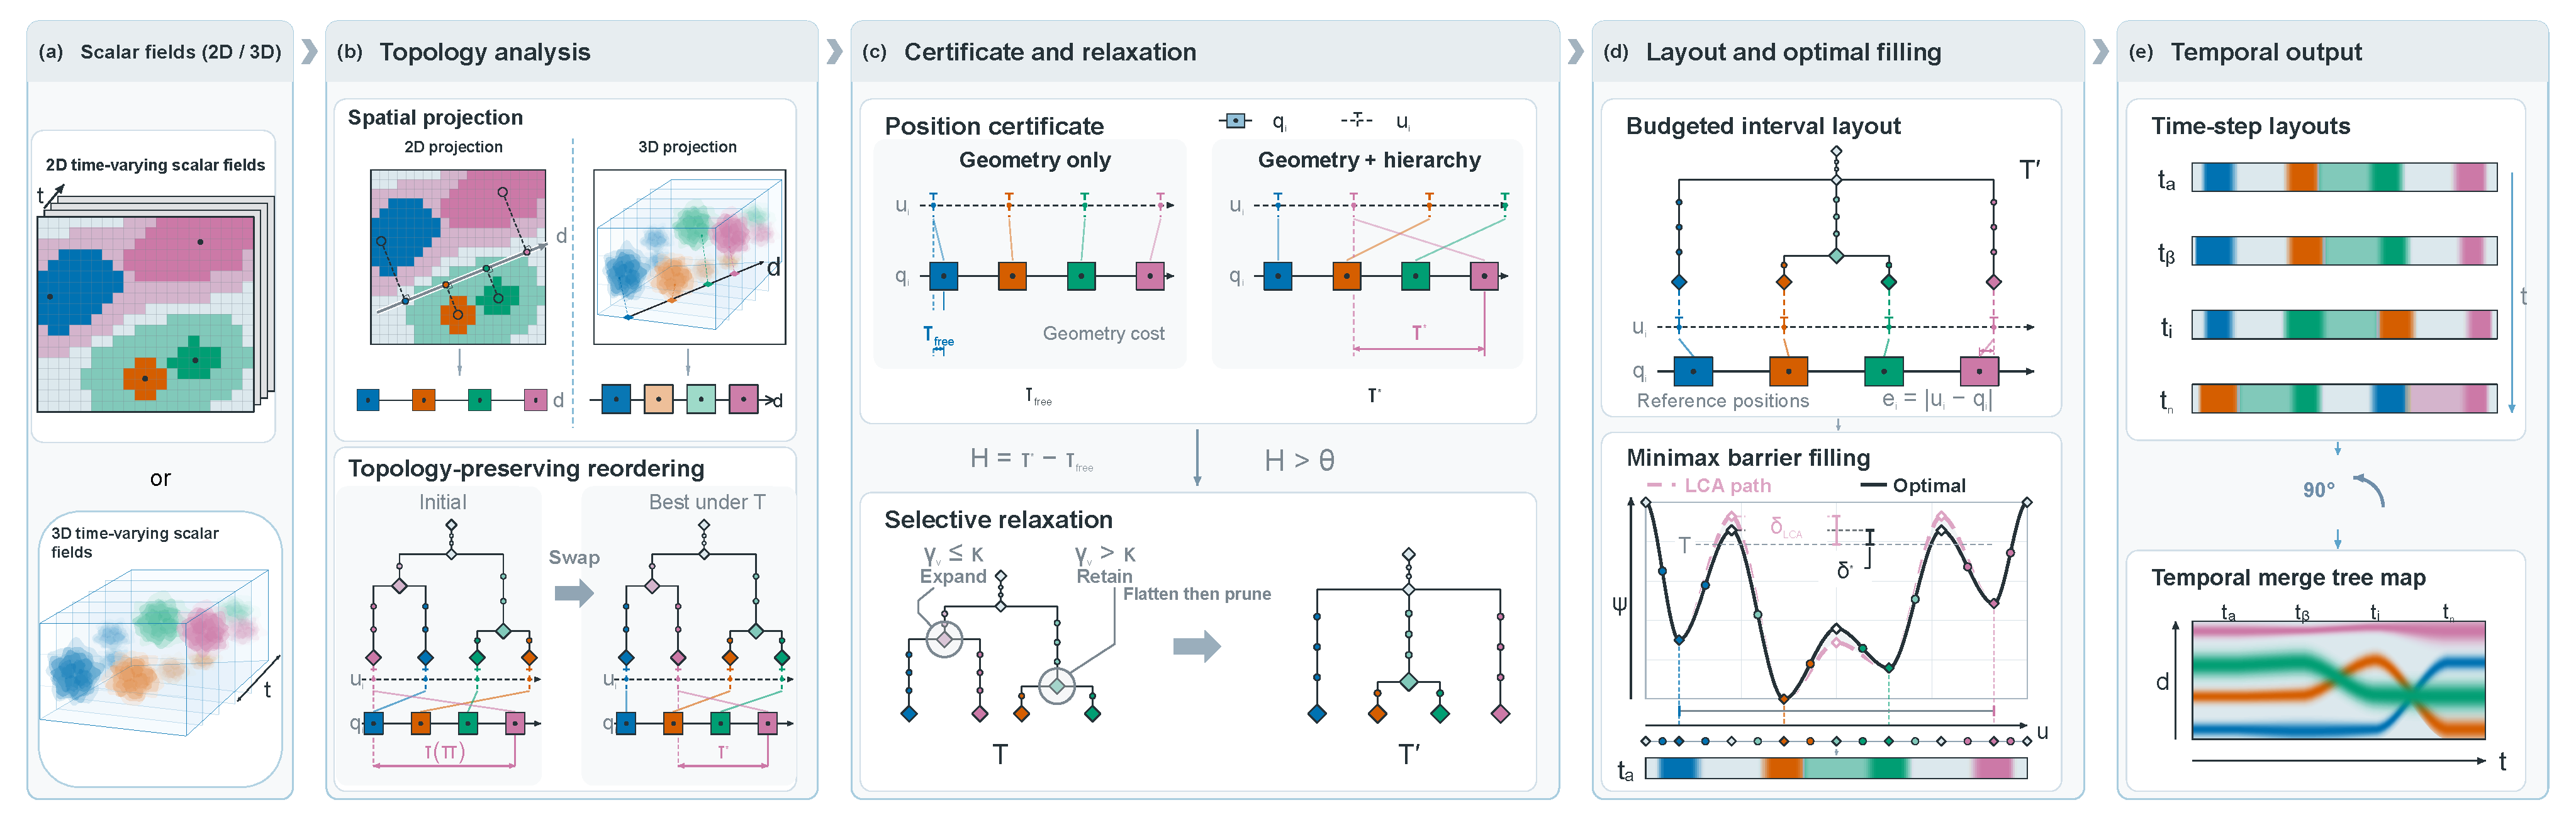
\includegraphics[width=\textwidth]{figures/Fig3.pdf}
\caption{RG-MTM's five stages (a)--(e), using the supplied four-feature schematic. Trees and a fixed projection define source merge targets and reference positions. Certificates diagnose hierarchy-dependent displacement; selective relaxation expands the ordering tree. Budgeted intervals and minimax filling construct profiles, stacked through time. The four branch identities retain blue, orange, green, and purple across stages; actual maps encode scalar values. Flatten-then-prune restoration is used in the planar protocol. $\kappa$ controls eligibility; output barriers determine measured cost.}
\label{fig:pipeline}
\end{figure*}

Figure~\ref{fig:pipeline} follows the data from scalar-field input through topology and projection, certificate-driven hierarchy choice, interval layout with optimal filling, and temporal assembly. The construction uses the source tree for scalar targets throughout; the ordering tree controls the permutations available to the layout.
Algorithm~\ref{alg:rgmtm} collects the construction and its hierarchy-selection and barrier routines in one procedure. Its inputs are augmented trees and tracked features from the extraction stage; its output records both the map and the achieved errors.
\begin{algorithm}[t]
\caption{Reference-guided temporal merge tree maps.}\label{alg:rgmtm}
\small
\algrenewcommand{\algorithmicrequire}{\textbf{Data:}}
\algrenewcommand{\algorithmicensure}{\textbf{Result:}}
\algrenewcommand{\algorithmicfunction}{\textbf{Function}}
\begin{algorithmic}
\Require Augmented trees $T_t$, extrema, supports, matches, domain $\Omega$; mode P/R and parameters $\theta,\kappa,\beta,\mathcal G$
\Ensure Temporal map $\mathcal V$; position bounds, anchor residuals, and measured merge errors
\Function{BuildMap}{$\{T_t\},\mathrm{matches},\mathrm{mode}$}
 \State $(d,q,[a,a+L])\gets\Call{SharedReference}{\mathrm{extrema},\mathrm{matches},\Omega}$
 \For{each time step $t$}
  \State Set support widths and check packing on $[a,a+L]$
  \State $(\mathcal D_t,\underline H_t)\gets\Call{Diagnose}{T_t,q_t,\mathcal G_t}$
  \State $T'_t\gets\Call{ChooseTree}{T_t,\underline H_t,\mathrm{mode}}$
  \State $\overline\tau'_t\gets$ feasible certificate upper bound for $T'_t$
  \State $B_t\gets\overline\tau'_t+\beta$
  \State $\mathcal C_t\gets$ budget-feasible legal orders of $T'_t$: enumerate for small trees; at most four candidates for large trees
  \State $(\pi,z,u)\gets$ best feasible layout from candidate QPs, using the preceding frame's matched layout
  \State $(v_t,\alpha)\gets\Call{RasterizeAndFill}{T_t,\pi,z,u}$
  \If{$T'_t\ne T_t$}
   \State $(b,\delta^*)\gets\Call{OptimalBarriers}{\pi,T_t}$
   \State Correct $v_t$ to barriers $b$ with strict-extremum clearance; retain anchor values at $\alpha$
  \EndIf
  \State Record $\mathcal D_t$, anchor residuals, and merge error measured from $v_t$ against $T_t$
 \EndFor
 \State \Return columns $[v_1\ \cdots\ v_K]$ with shared scalar colors
\EndFunction
\Statex
\Function{ChooseTree}{$T,\underline H,\mathrm{mode}$}
 \If{mode P or $\underline H\le\theta$} \State \Return $T$ \EndIf
 \State $W\gets$ non-root branching nodes with $\gamma_v\le\kappa$
 \State $T'\gets\mathrm{flat}(T,W)$
 \If{planar protocol}
  \State $b_0\gets$ grid-certificate score of $T'$
  \State Restore constraints in $T'$ by decreasing $\gamma_v$ while its score stays within half a pixel of $b_0$
 \EndIf
 \State \Return $T'$
\EndFunction
\Statex
\Function{OptimalBarriers}{$\pi,T$}
 \If{fewer than two leaves} \State \Return no barriers, $0$ \EndIf
 \State Renumber leaves by $\pi$; obtain original LCA levels $M_{ij}$
 \State $C_k\gets\min_{i\le k<j}M_{ij}$ for each inter-anchor gap $k$
 \State $\delta\gets\max(0,\max_k[\max(f_k,f_{k+1})-C_k])$
 \For{each leaf pair $i<j$}
  \State $\delta\gets\max\bigl(\delta,[M_{ij}-\max_{i\le k<j}C_k]/2\bigr)$
 \EndFor
 \State \Return $C+\delta$, $\delta$
\EndFunction
\end{algorithmic}
\end{algorithm}


\subsection{Shared Reference and Diagnosis}\label{sec:reference}
\textsc{SharedReference} derives one sequence-wide direction from consecutive-frame matches. It accumulates the outer products of matched extremum displacements, takes the leading unit eigenvector, and orients its sign toward the total displacement. Projecting retained extrema and domain corners then fixes the reference coordinates and canvas for all columns. A supplied direction supports a selected geographic axis. Feature widths use area or volume with the same conversion factor over the sequence.

\textsc{Diagnose} assigns each frame position costs, hierarchy cost, and conflict triples. Exact small-tree evaluation returns $\tau^*(T_t)$, $\tau_{\free,t}$, and $H_t$; a bounded large-tree evaluation retains lower and upper endpoints for both position costs. Its nonnegative hierarchy lower bound is $\underline H_t=\max(0,\underline\tau^*(T_t)-\overline\tau_{\free,t})$, which coincides with $H_t$ when both costs are exact. The gate uses this lower bound; layout uses a feasible positional upper bound. Conflict triples identify which feature relations exclude the desired order.

\subsection{Preserving and Relaxed Ordering Trees}\label{sec:relaxation}
RG-MTM-P sets $T'_t=T_t$. RG-MTM-R activates when $\underline H_t>\theta$ and marks non-root branching nodes with $\gamma_v\le\kappa$ as eligible. Flattening these nodes joins their child blocks to their parent and permits additional interleavings while retaining all leaves. The original merge targets remain in $T_t$.

For the two-dimensional suite, restoration removes unnecessary flattenings. Compute the grid-certificate score $b_0$ after flattening every eligible node. Visit nodes in decreasing merge-gap order and restore a constraint whenever its score stays within half a pixel of the fixed $b_0$. The resulting tree retains the original constraints that fit the initial relaxed position score. Volumetric construction retains the eligible flattenings and uses the large-tree search described below.

Shared settings use $c|\Omega|=L/2$, $\rho=0.5$, $g=L/240$, $\beta=L/120$, and $\theta=0.02L$, with domain area or volume for $|\Omega|$. The main planar temporal setting is $\kappa=0.2\Delta_F$, where $\Delta_F$ is the fixed processed scalar range. We abbreviate eligibility fractions 2\%, 20\%, and 100\% as R2, R20, and R100. This threshold selects eligible parent gaps; it does not cap the rendered merge-level error. \textsc{OptimalBarriers} computes the selected order's scalar cost. The static and volumetric protocols retain their declared simplification, candidate-search, and relaxation settings (Supplement S6 and S9).

\subsection{Budgeted Interval Layout}
The position budget $B_t=\overline\tau'_t+\beta$ uses a feasible positional upper bound and reserves allowance for geometric and temporal objectives; exact diagnosis gives $\overline\tau'_t=\tau^*(T'_t)$. For each budget-feasible legal order, a convex quadratic layout combines four mean squared residuals: anchor-reference offsets (weight 4), ordered anchor distances versus support-centroid distances (1), matched projected-motion residuals (0.5), and anchor eccentricities (0.1). The motion residual subtracts the projected source displacement from the matched anchor displacement. The interval geometry and $|u_i-q_i|\le B_t$ constrain the coordinates; the smallest evaluated objective selects the layout sequentially through time.

Small-tree construction enumerates legal orders and evaluates their continuous position costs. Large-tree construction propagates continuous earliest-finish Pareto functions through low-degree nodes; higher-degree cases use workload bounds or a time-limited mixed-integer program. Each result retains a lower bound, a feasible upper bound, and a witnessing order. Layout uses the upper bound plus $\beta$ and evaluates up to four legal candidates assembled from the certificate, reference-preferred, temporal-preferred, and TMTM orders. Fixed-order convex QPs record feasibility and first-order objective gaps. Figure~\ref{fig:pipeline} summarizes the construction; Supplement S1 details the planar construction and S6 the volumetric solver protocol.

\paragraph{Guarantees and selection.}
For a fixed order, the position cost and non-strict scalar cost are exact quantities of the display model. Exact small-tree enumeration also resolves the attainable frontier. The constructed map instead selects a secondary objective within a feasible position budget; a finite large-tree candidate set does not establish global optimality over all legal orders. Certificate intervals disclose unresolved position costs, and measured anchor and barrier errors describe the actual output. This distinction applies equally to preserving and relaxed modes.

\subsection{Scalar Filling and Temporal Assembly}\label{sec:domain_filling}
\begin{figure}[t]
\centering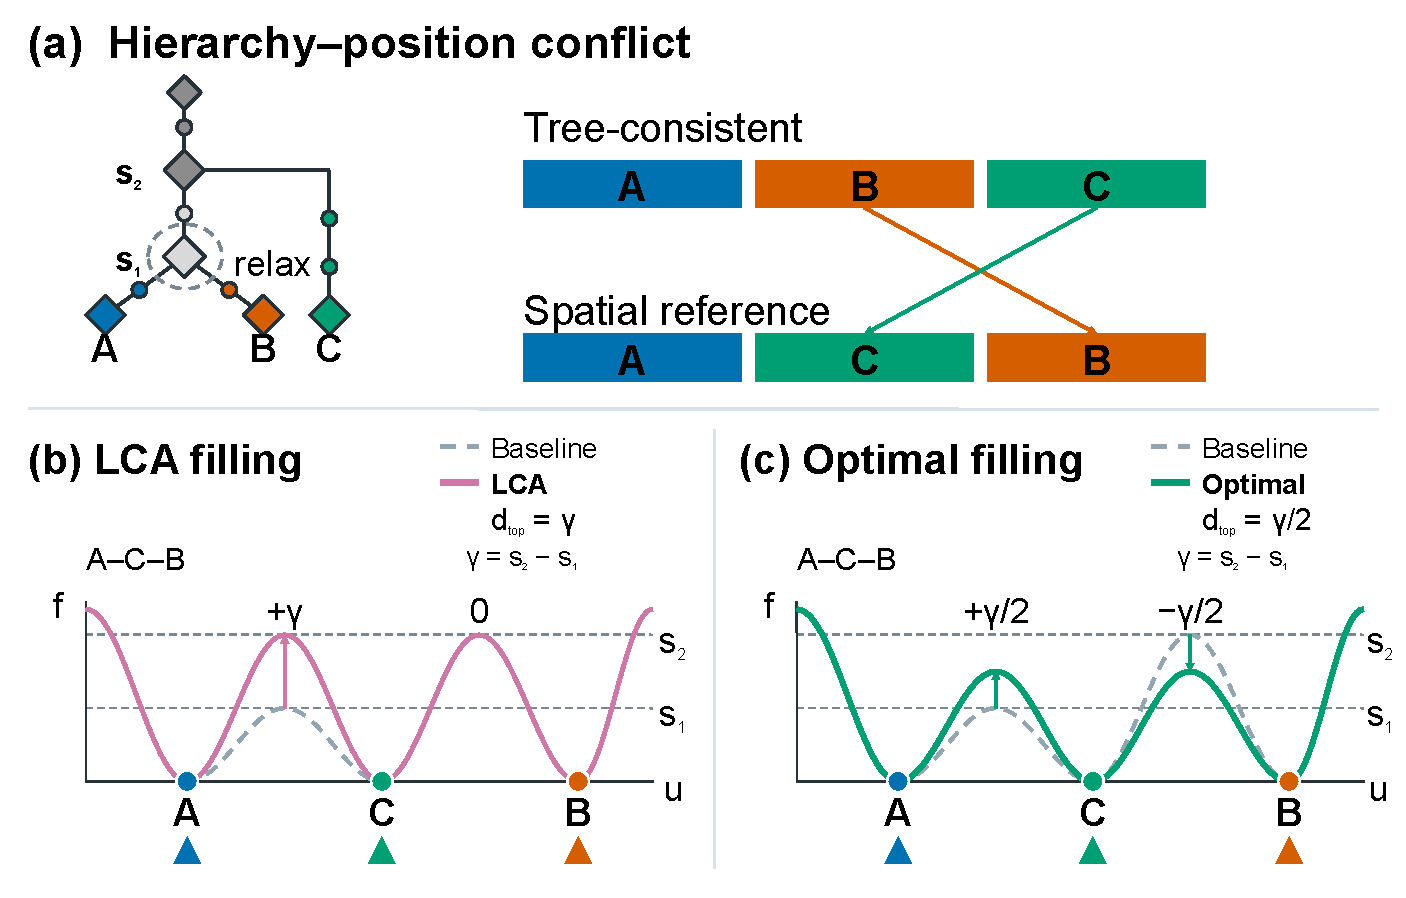
\includegraphics[width=\linewidth]{figures/Fig4.pdf}
\caption{Hierarchy--position conflict and scalar filling for three equal-valued minima. (a) The source tree groups $A,B$, excluding reference order $A,C,B$. Identity colours match the other schematics: $A$ blue, $B$ orange, and $C$ green. (b,c) Both fillings use the same relaxed anchors in order $A,C,B$, with identical reference triangles. Original-LCA filling (purple) sets both barriers to $s_2$, incurring $d_{\rm top}=\gamma=s_2-s_1$. Optimal filling (green) places both at $(s_1+s_2)/2$, attaining $\gamma/2$ when fixed leaf values lie below this level. The dashed grey baseline retains the hierarchy and its anchor displacement. Curves are schematic.}
\label{fig:filling}
\end{figure}

Scalar filling reuses ST-MTM's leaf-arc and hierarchical-path construction~\cite{STMTM:2026}. True extremum values occupy the anchors; resampled arc values alternate around them. Inter-anchor gaps follow original-tree LCA paths, allocating sibling, direct--deep, and deep--deep cases according to their arc lengths. Root paths fill the borders; Supplement S2 details each case.
\textsc{RasterizeAndFill} denotes this initial rendering on the shared canvas. \textsc{OptimalBarriers} uses join-tree values; split-tree values are negated before correction and transformed back afterwards. Its returned $\delta^*$ is the analytical fixed-order cost; measured raster error is recorded after clearance and filling.

RG-MTM-P retains the original merge barriers. For a relaxed order, call \textsc{OptimalBarriers}, clip each inter-anchor segment at its returned barrier, and raise its peak to that level when needed. Endpoint extrema retain their values. Figure~\ref{fig:filling} separates the order change from its scalar correction. The source tree $((A,B),C)$ excludes reference order $A,C,B$. For that relaxed order, original-LCA filling sets both inter-anchor barriers to $s_2$, changing the $A/B$ merge by $\gamma=s_2-s_1$. Optimal filling balances the three pairwise discrepancies at $\gamma/2$ by placing both barriers at $(s_1+s_2)/2$, provided the fixed leaf values lie below that midpoint. The dashed grey preserving profile shows the anchor displacement removed by the new order; the purple and green curves isolate filling quality at the same relaxed anchors.

The renderer maps the fixed canvas to the same raster coordinates at every time step and stacks columns chronologically. Shared colours encode scalar values; matched extrema form temporal tracks. Each frame records its position certificate, achieved anchor residuals, and actual merge-level error measured from the filled column. Nearest-pixel anchor rounding contributes at most $L/[2(N-1)]$ for raster length $N$, with capacity checked before filling.
